%% stevensthesis_num.tex
%% Copyright 2008 B. E. Arnett
%
% This work may be distributed and/or modified under the
% conditions of the LaTeX Project Public License, either version 1.3
% of this license or (at your option) any later version.
% The latest version of this license is in
%   http://www.latex-project.org/lppl.txt
% and version 1.3 or later is part of all distributions of LaTeX
% version 2005/12/01 or later.
%
% This work has the LPPL maintenance status `maintained'.
% 
% The Current Maintainer of this work is Barbara Arnett.
%
% This work consists of the files stevensthesis_num.tex 
% and the derived file pgnumchapter_nums.sty.

%
% This is the template for dissertation / thesis submission for the
% Stevens Institute of Technology.  
%
% There are fields in titlepg.sty that must be updated with your
% own information.  The file pgnumchapter.sty must be included but  
% does not need to be updated, unless you want to change the 
% layout of your pages and chapters.  
%
% Both dissertations and master thesis can created from this program.  
% These fields should be changed:
%    {thesistype} should be either "dissertation" or "thesis" 
%    {thesisdegree} should be either "doctor of philosophy" for dissertation or
%            "Master of Engineering - Electrical Engineering" 
%            "Master of Science - Computer Science"   or the correct degree designation.
%
%
% Please see the formatting instructions on the library website at
%        http://www.stevens.edu/services/thesis.html
%
% copyright 2007, Barbara Arnett, web services librarian, stevens institute of technology
% any comments or corrections can be sent to barnett@stevens.edu
%
% update January 2009 - updated font size to 12p and added subsections to show up in the 
% table of contents 
%
%
%

\documentclass[12pt]{report}
\usepackage {fancyhdr}
\usepackage{graphicx, amssymb}
\usepackage{setspace}
\usepackage{pgnumchapter_nums}
\usepackage{listings}
\usepackage{titlepg}
%              this is for the list of symbols page, if desired
\def\listofsymbols{%   This is the file for symbols used in the paper.
%
%\addnotation \alpha: {some variable that means something to me}{alpha}
%\addnotation \Omega: {abstract probability space}{alpha}


%%%%%%%%%%%%%%%%%%%%%%%
%Sample List of Symbols
%%%%%%%%%%%%%%%%%%%%%%%
\begin{tabbing}
% YOU NEED TO ADD THE FIRST ONE MANUALLY TO ADJUST THE TABBING AND SPACES
\hspace{5mm}$n$~~~~~\=\parbox{5in}{Vector size\dotfill \pageref{symbol:nml}}\\
%ADD THE REST OF SYMBOLS WITH THE HELP OF MACRO
\hspace{5mm}\addsymbol m: {Vector size}{symbol:nml}
\hspace{5mm}\addsymbol l: {Vector size}{symbol:nml}
\hspace{5mm}\addsymbol x: {State vector}{symbol:x}
\hspace{5mm}\addsymbol u: {Control input}{symbol:x}
\hspace{5mm}\addsymbol y: {Output vector}{symbol:x}
% .
% .
% .
\hspace{5mm}\addsymbol \mathbf{A}: {State Matrix}{symbol:A}
\hspace{5mm}\addsymbol \mathbf{B}: {Input Matrix}{symbol:B}
\hspace{5mm}\addsymbol \mathbf{C}: {Output Matrix}{symbol:C}
% .
% .
% .
% ALWAYS KEEP THE FOLLOWING LINE
\end{tabbing}
 \clearpage}
\def\addsymbol #1: #2#3{$#1$\> \parbox{5in}{#2 \dotfill  \pageref{#3}}\\}
\def\newnot#1{\label{#1}}

\pagestyle{fancy}
\fancyhead[LE,RO]{helv \thepage}

\doublespacing

\lhead{}
\chead{}
\rhead{\thepage}
\lfoot{}
\cfoot{}
\rfoot{}

\renewcommand{\headrulewidth}{0  pt}          %this prints a line under the header
\renewcommand{\footrulewidth}{0  pt}            %this prints a line under the footer


\renewcommand{\contentsname}{\normalsize{Table of Contents}}
\renewcommand{\listfigurename}{\normalsize{List of Figures}}
\renewcommand{\listtablename}{\normalsize{List of Tables}}
\renewcommand{\bibname}{\normalsize{Bibliography}}
\renewcommand{\indexname}{\normalsize{Index}}
\renewcommand{\thesubsection}{\thesection\arabic{subsection}}





%%

%%
%\renewcommand{\section}{\normalsize{\section}
%\newcommand\figurename{Figure}
%\newcommand\tablename{Table}
%\newcommand\partname{Part}
%\newcommand\chaptername{Chapter}
%\newcommand\appendixname{Appendix}
%\newcommand\abstractname{Abstract}


% you may need to change the pdfpagewidth to pagewidth
% and pdfpageheight to pageheight

% if not using pdflatex to produce output, you may need to change to pagewidth and pageheight variables.
%\pagewidth 8.5in
%\pageheight 11in 
\pdfpagewidth 8.5in
\pdfpageheight 11in 
%
\setlength{\textheight}{8.5in} 
\setlength{\oddsidemargin}{0.5in}  
\setlength{\evensidemargin}{0.5in} 
\setlength{\textwidth}{6.0in}
\setlength{\topmargin}{0.0in} 
\setlength{\headheight}{0.25in}
\setlength{\headwidth}{6.0in}
\setlength{\headsep}{0.25in}
\setlength{\parindent}{12mm}


%%%%%%%%%%%%%%%%%%%%%%%%%%%%%%%%%%%%%%%%%%%%
%%%
%%%  This begins the frontmatter of the document, everything preceding the body 
%%%
%%%%%%%%%%%%%%%%%%%%%%%%%%%%%%%%%%%%%%%%%%%%


\begin{document}



\pagenumbering{roman}

\thesistitlepage

\thesiscopyrightpage              

\thesisabstract

% \thesisdedicationpage

% \thesisacknowledgements

\tableofcontents

\listoftables

\makeatletter \renewcommand{\@dotsep}{10000} \makeatother    %removes dots before page numbers

\listoffigures

%%%
%    this produces the list of symbols.  the dots have been left in to show how it would look with dots.  The formatting of the table of contents, list of symbols 
%    and list of figures is up to the author, but they should all match and be similar in format.    The list of symbols is optional, it can be un-commented
%    out if desired.
%%% 
%   \newpage
%   \chapter*\normalsize\textbf{List of Symbols\hfill} %   \addcontentsline{toc}{chapter}{List of Symbols}
%   \listofsymbols


%%%%%%%%%%%%%%%%%%%%%%%%%%%%%%%%%%%%%%%%%%%%
%%%
%%%  This begins the body of the document
%%%
%%%%%%%%%%%%%%%%%%%%%%%%%%%%%%%%%%%%%%%%%%%%


\newpage
\pagenumbering{arabic}


\chapter{Introduction} % (fold)
\label{cha:introduction}
Evolution has classically been a science of the past. That is, the primary sources of evidence used in the formulation and validation of evolutionary theory have been the fossil record, geology, and observations of the current form and distribution of species as a result of events that took place in the past. Where evolution does exhibit predictive power, it is primarily in the ability to predict what new evidence from the past should eventually be revealed, such as the many fossils of transitional forms discovered over the past centuries. In this regard, evolution has been wildly successful.

Where the study of Evolution has been thus far lacking is in its ability to predict the future. That is, looking at a collection of fossils and historical records of environmental conditions, evolutionary theory gives us the ability to identify which selective pressures acted on past populations. What evolutionary theory cannot do, at present, is predict which environmental conditions or physical forms will act as selective pressures in the future. At best, we can make educated guesses based on past evidence, but we lack the ability to assign a concrete measure of confidence in such predictions. In the end, the only sure way to determine which individuals are best fit is to wait and see which individuals ultimately survive and reproduce.

This is not an inherent failing of evolution, but rather a sign of a young and developing field. The inability to predict the future course of evolution is tied directly to the fact that selective pressures can come from practically any feature of an organism. Everything from diet to behavior to physical form can lead to a selection for or against the eventual reproductive success of an organism. The situation in which evolution finds itself is akin to what physics would be like if every projectile had its own unique laws of motion. What evolution desperately needs is a fundamental set of principles from which the success of any organism can be derived, much as the path of every projectile can ultimately be derived from Newton's laws of motion.

The implications of a coherent method for deriving the evolutionary success of an individual undergoing natural selection would be far reaching. Perhaps the most obvious implication would be an improved ability to predict patterns of disease emergence and transmission. Cancer treatment would be another potential area of benefit, as cancer is an evolutionary process. With each round of chemotherapy or radiation treatment, those cancer cells which are better adapted to resist treatment will survive. These cells will then seed a reemergent, more difficult to treat, tumor. Understanding the dynamics of evolution, and how to predict the future course of evolution, would improve our ability to design effective treatments for both microbial diseases and cancer.

Even non-biological processes are driven by evolution and obey many of the same laws that Darwin first laid out 150 years ago. Both languages and economies undergo evolutionary processes, driven by the same math as cancer or the origin of species\cite{ANowak:2006p857}. That said, we must make a distinction between biological and non-biological evolution. The reason for doing so lies in the approaches that can be taken to investigate each type of evolutionary system. We know far more about biological organisms than merely that they evolve. The past 50 years has seen an explosion of knowledge about the chemistry of life and the operation of those molecular systems which compose cells and influence the phenotypes of complex multicellular organisms.

For this reason, biological systems undergoing evolution present a unique opportunity to attempt to derive the fundamental principles of evolution from the individual mechanics of the evolving systems. Specifically, with biology we can explore the feedback mechanism which drives evolution: the ``Central Dogma'' of biology. This is the pathway by which information flows from an organism's nucleic acids, where it is stored, to the organism's proteins which then drive fundamental biochemical processes\cite{Thieffry:1998p913}. These biochemical processes determine the phenotypes eventually selected for or against in the process of natural selection. From this flow of information, it is understood that those organisms which contain the information for generating the better fit traits will become enriched in the population, and therefore will pass on this information in greater numbers than their less fit peers\cite{Darwin:1883p935}.

The biochemical processes that ultimately result in phenotypic traits can be very complex, and their ultimate effect may be indirect. This makes it difficult to study the biochemical evolution of all but the simplest of traits in the simplest of organisms. There is, however, at least one biochemical process that is relatively simple, and whose impact has a very direct effect on the eventual transmission of genetic information: the process of nucleotide synthesis. Since a prime requirement for reproduction, especially in an era when all life was unicellular, is the ability to replicate genetic information, one would expect this to be a process under heavy selective pressure. Also, since the phenotype of reproduction rate is very closely tied to and dependent upon the specific molecular mechanisms, this process provides a prime opportunity to study how organism-scale selection manifests itself at the molecular scale.

\section*{Nucleic Acid Polymerization} % (fold)
\label{sec:nucleotide_polymerization}
The two classes of biologically important nucleic acids are Ribonucleic Acid (RNA) and Deoxyribonucleic Acid (DNA). These two classes are very similar, differing only by the presence or absence, respectively, of a 2' hydroxyl group on the ribose sugar of their individual monomers and the specific nitrogenous bases attached at the 1' position. Both types of polymer are formed by a process of dehydration synthesis catalyzed by a class of enzymes known as nucleotide polymerases. The dehydration reaction takes place between one of the hydroxyl groups on the $\alpha$-phosphate of a nucleotide triphosphate and the 3' hydroxyl group of the terminal monomer on the growing nucleic acid chain\cite{ZannisHadjopoulos:1999p952}.

What is phenomenal about this process is that, first, it occurs in all biological organisms and, second, that it always occurs in the same manner. To understand why the consistency of directionality is notable, it helps to understand the catalytic process that occurs at the active center of nucleotide polymerases. All known nucleotide polymerases share a common chemical mechanism. In this mechanism two divalent metal cations, coordinated by a number of acidic amino acids, facilitate the transfer of an electron pair from the free 3' hydroxyl group of one nucleotide to the $\alpha$ phosphate, which is attached to the 5' hydroxyl of the other nucleotide\cite{Castro:2009p953} (see Figure~\ref{fig:reactions}).

\begin{figure}[h]
	\centering
		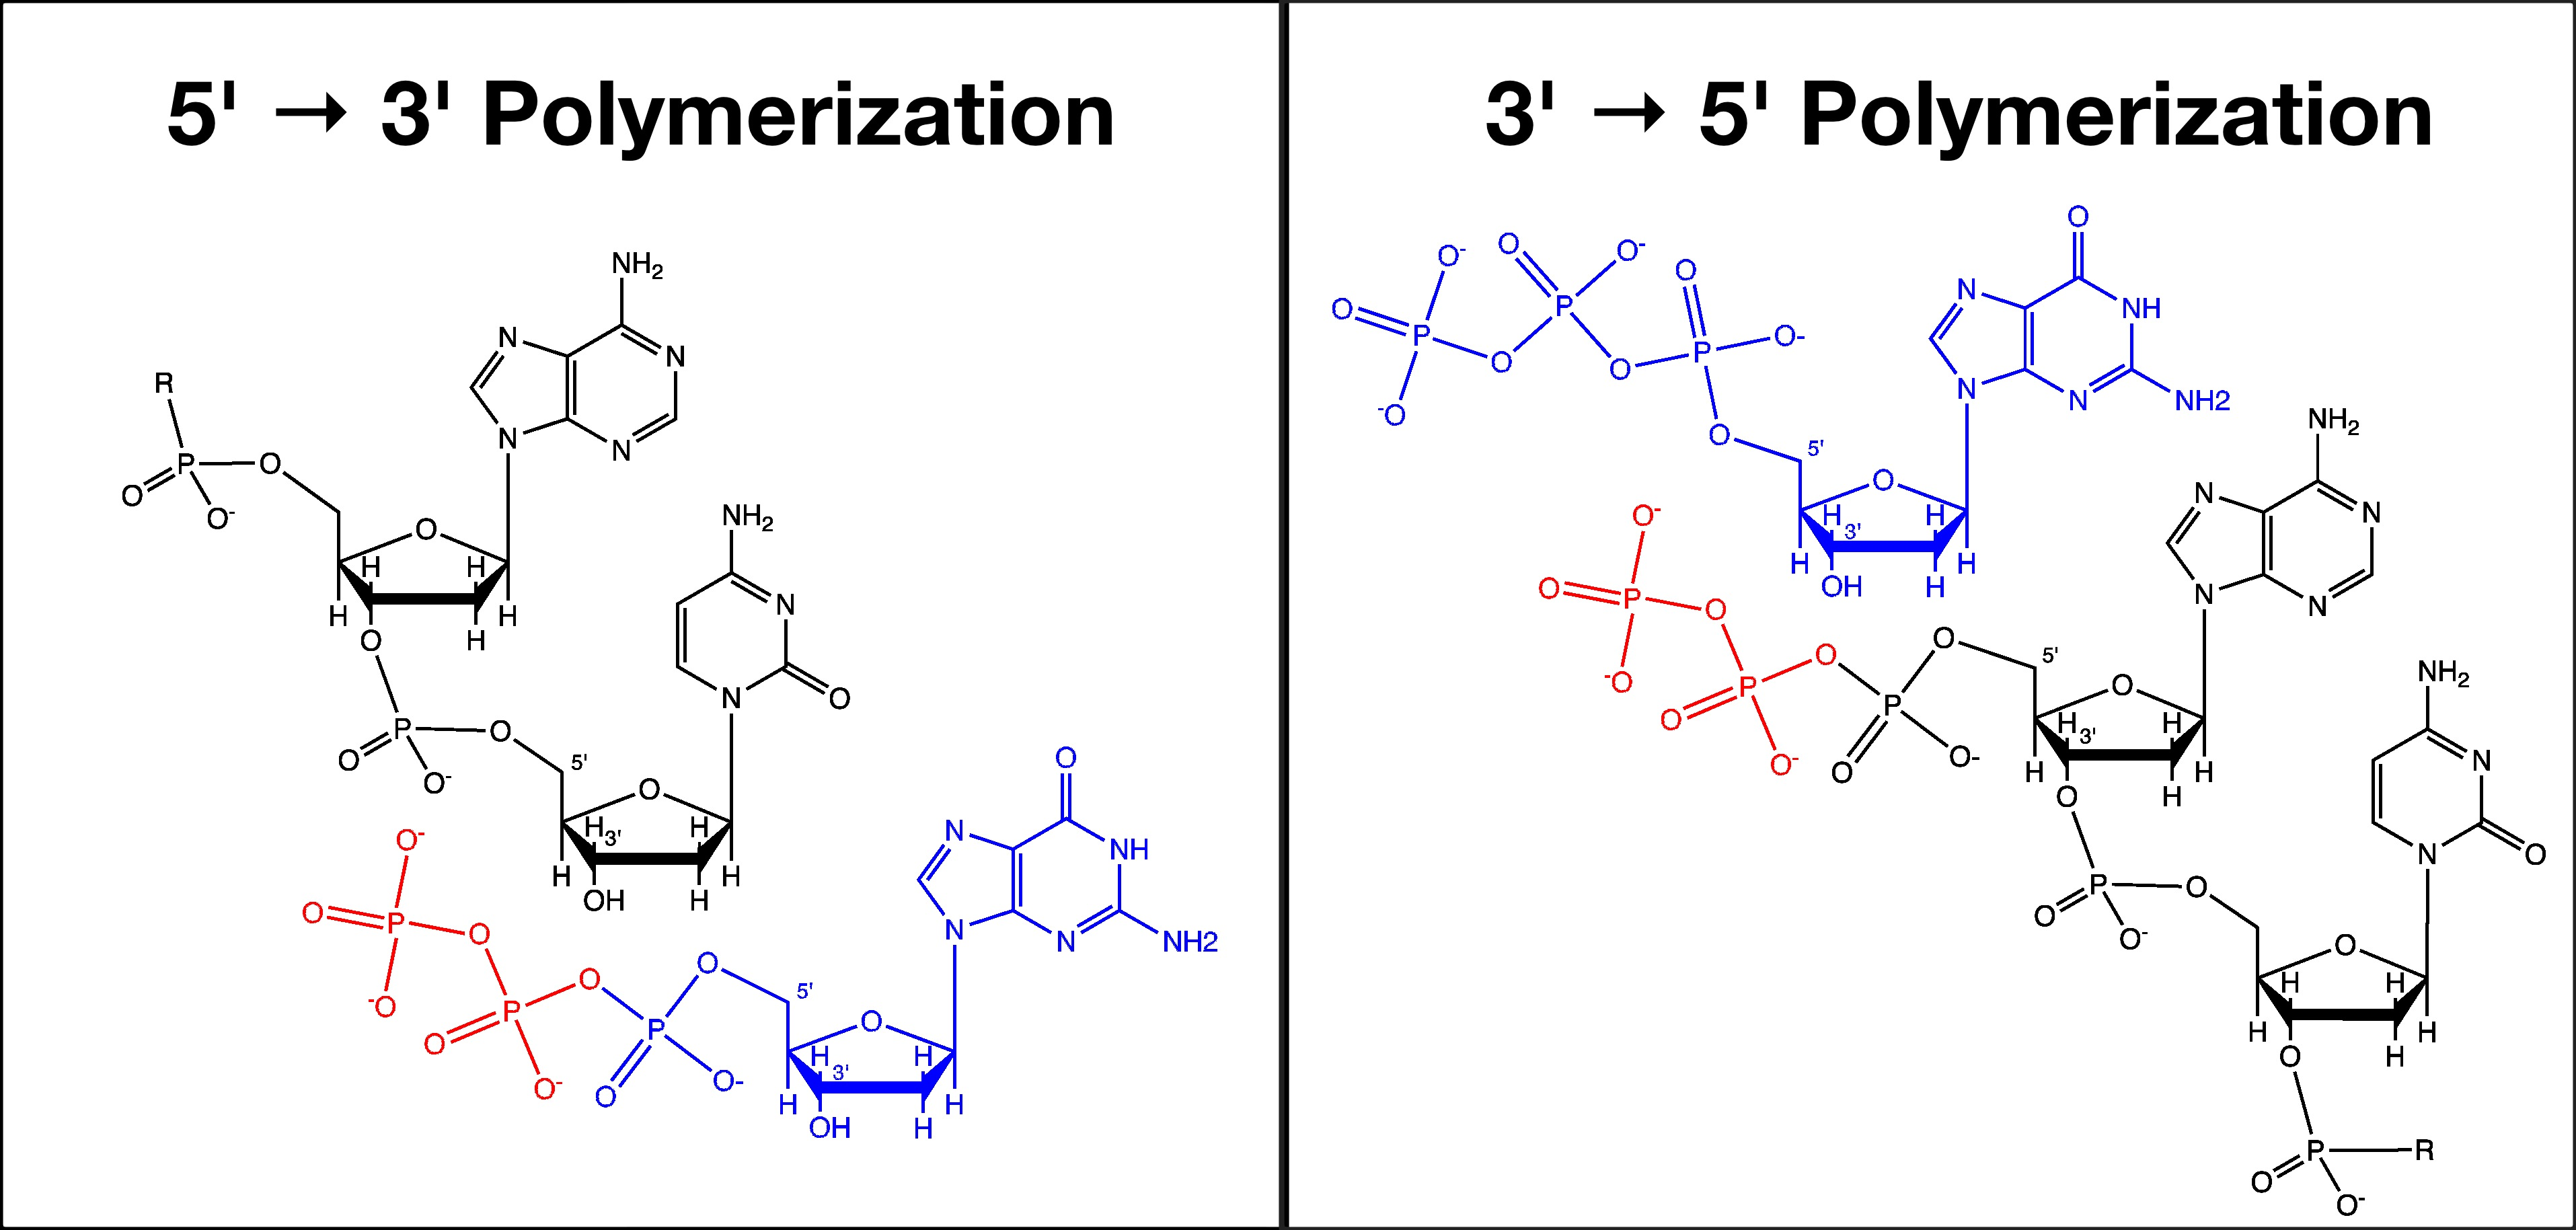
\includegraphics[width=\textwidth]{reactions}
	\caption{\textbf{Schematic of the Known $5'\to3'$ and the Proposed $3'\to5'$ Polymerization Reactions.} In each panel, the incoming nucleotide is colored blue and the pyrophosphate leaving-group is colored red. The 3' and 5' carbon atoms on the sugars of the incoming nucleotide and the terminal nucleotide of the growing chain are labeled (R represents the remainder of the growing polymer). Note that the pyrophosphate leaving-group is found on the incoming nucleotide in the $5'\to3'$ reaction, but the leaving-group in the $3'\to5'$ reaction is on the growing chain itself.}
	\label{fig:reactions}
\end{figure}

Importantly, the catalytically active cations of the polymerase active site have no knowledge of whether the 5'-phosphate is attached to the incoming nucleotide or the growing chain. If one were to imagine a nucleotide polymerase that proceeded in the reverse direction of all currently known nucleotide polymerases, the only aspect of the naturally occurring enzymes that would need to be modified are those portions which attach to the growing nucleotide polymer or the incoming nucleotide, all of which are distinct from the catalytic center. That is, there should be nothing preventing the chemical reaction at a hypothetical $3'\to5'$ polymerase active site from occurring.

The fact that all biological organisms polymerize both DNA and RNA with the same directionality implies that this aspect of nucleotide polymerization was decided extremely early on in the genesis of life on earth, most likely even before the biological distinction between DNA and RNA functionality arose. If the active site mechanism of nucleotide polymerases cannot explain the bias of all life toward one polymerization directionality over the other, what alternative explanations might exist? There are two possibilities. The first is that the unique directionality is the consequence of a founder effect. A founder effect is when a small subset of a larger population is evolutionarily isolated and goes on to give rise to a new population. This new population would be expected to contain an oversampling of the traits of the small founding population as compared to the gene frequencies of the original population\cite{Templeton:1980p954}. In the case of nucleotide polymerization, this would imply that at some point early on in the development of life on earth the population contained both forms of nucleotide polymerase, those that polymerize by extension $3'\to5'$ and $5'\to3'$. Then, at some later point a subgroup of this population, consisting entirely of organisms with a $5'\to3'$ polymerase, was isolated and subsequently gave rise to all life on earth today.

The other possibility is that there is an evolutionary advantage to the $5'\to3'$ directionality, and that all life polymerizes nucleotides in this direction as the result of a selection event. Unfortunately, the chances of finding any evidence directly supporting the hypothesis of a founder effect determining polymerase directionality are essentially nil. Short of finding some remnant modern population with reversed polymerases, the only evidence of an ancient $3'\to5'$ polymerase would be the enzymes or other early replicator molecules themselves, and individual molecules do not fossilize. The only way to shed light on which of these two competing hypotheses explains the current state of nucleotide polymerases would be to identify an evolutionary advantage imparted by a $5'\to3'$ polymerase over the reverse.

What might be the source of such an advantage? Looking again at the chemical reactions that would be carried out in each case (fig.~\ref{fig:reactions}), a major difference between the $5'\to3'$ case and the $3'\to5'$ case is the location of the pyrophosphate leaving-group relative to the other components of the polymerization reaction. This is important because it is known that triphosphate groups attached to nucleotides can spontaneously hydrolyze\cite{Sigel:1983p720}. In the event that the triphosphate leaves prematurely with the $5'\to3'$ polymerase, it would be possible for the enzymatic machinery to discard the (now useless) incoming nucleotide and replace it with a new nucleotide containing an active triphosphate. In the event of a spontaneous hydrolysis with the $3'\to5'$ polymerase, because the active triphosphate in the reaction is on the growing chain the only choice the enzymatic machinery has is to discard all of its progress thus far or wait for some secondary machinery to replace the triphosphate group. Given that the former of these two choices represents significant waste, we can assume that the later choice is the only one that would be even remotely sustainable, but this choice involves introducing a delay in reproduction.

A delay, on its own, does not necessarily mean that the $3'\to5'$ case is at enough of a disadvantage to be completely eliminated from a population through natural selection. After all, polymerase rates are variable and a hypothetical $3'\to5'$ polymerase could simply evolve to polymerize faster. Unfortunately, such modifications come with a cost. There is a relationship between speed of nucleotide polymerization and error rate\cite{Griep:2006p719}, and polymerizing faster would cause the polymerase to make more mistakes. A higher frequency of errors during reproduction would introduce a higher rate of mutation, making it more difficult for the $3'\to5'$ polymerizing organisms to maintain their speed advantage. Again, on its own this is not reason enough to dismiss the possibility of a $3'\to5'$ polymerase. There are many factors at play, and to understand how all of these combined contribute to the fitness of an organism that synthesizes its nucleic acids in a $3'\to5'$ direction, we will need to model the competitive evolution of the two polymerase types.
% section nucleotide_polymerization (end)

\section*{Modeling Evolution} % (fold)
\label{sec:modeling_evolution}
Because nucleotide polymerases are responsible for replicating the genetic information of an organism, and have a direct influence on both the rate at which an organism can reproduce as well as the fidelity with which genetic information is conveyed from one generation to the next, the approach I will take is relatively straightforward. The model presented here involves simplified model organisms designed to represent the earliest forms of self-replicating life. It is assumed these organisms exist in an environment rich with nutrients and an excess of available energy. The result of this being that the rate of genome duplication serves as the lone limiting factor on reproductive rate.

Since polymerase directionality would have been fixed extremely early on in the origin of life, it is reasonable to assume that the recombination of genetic elements would contribute only a negligible amount of variation to the model organisms. Additionally, the simplest of nucleotide polymerases observed in nature are the products of single genes. Even if there was recombination of individual genetic elements, the exclusive focus of this model is the polymerase. Whether a product polymerase gene is transferred intact to the offspring of one organism or transferred horizontally will not affect the conclusions that can be made. This is a result of the first assumption made that the model organisms have an excess of all resources aside from the polymerase. That is, whatever organism a polymerase may end up in, it will always be the single determining factor for both reproductive rate and genetic fidelity.

Ultimately, the goal of this model is to investigate the link between a well understood molecular process, nucleotide polymerization, and an evolutionary outcome, the selection for polymerase enzymes which proceed $5'\to3'$. If there are general rules to be found that govern the process of evolution all the way from the molecular level to the scale of entire organisms and even populations, hopefully starting with a simple model like the one presented here will serve as an important first step in their eventual discovery.
% section modeling_evolution (end)

% chapter introduction (end)
\chapter{Design of the Polymerase Evolution Model} % (fold)
\label{cha:design_of_the_polymerase_evolution_model}
This chapter provides a detailed description of the design of the model system used to investigate the question of the evolution of polymerase polarity. The goal of this model is to have organisms containing either a $5'\to3'$ or a $3'\to5'$ nucleic acid polymerase compete with each other in order to see which strategies are either evolutionarily dominant or evolutionarily stable. The model is also designed such that the influence of temperature on the outcome of this competition can be investigated.
\section*{Overview} % (fold)
\label{sec:overview}

% section overview (end)
% chapter design_of_the_polymerase_evolution_model (end)
\chapter{Experimental Results of Polymerase Modeling} % (fold)
\label{cha:experimental_results_of_polymerase_modeling}

% chapter experimental_results_of_polymerase_modeling (end)
\chapter{Analysis and Discussion of Model Results} % (fold)
\label{cha:analysis_of_model_results}

% chapter analysis_of_model_results (end)
\appendix
\chapter{Source Code} % (fold)
\label{cha:source_code}
Following is the Ruby source code for the four main classes and the executable Ruby script used to run simulations based on YAML input files.
\lstset{language=Ruby, numbers=left, basicstyle=\scriptsize \tt, showstringspaces=false, commentstyle=\tt}
\lstset{title=environment.rb}
\lstinputlisting{../../../Source/Evolver/lib/evolver/environment.rb}
\lstset{title=organism.rb}
\lstinputlisting{../../../Source/Evolver/lib/evolver/organism.rb}
\lstset{title=genome.rb}
\lstinputlisting{../../../Source/Evolver/lib/evolver/genome.rb}
\lstset{title=polymerase.rb}
\lstinputlisting{../../../Source/Evolver/lib/evolver/polymerase.rb}
\lstset{title=evolver}
\lstinputlisting{../../../Source/Evolver/bin/evolver}
% chapter source_code (end)


% The bibliography would be contained below.  The formatting for the bibliography is not provided here.  Formatting for references can be in the writing style 
% set by the advisor.  Common styles are APA, MLA and Chicago style. 
\bibliography{references}{}
\bibliographystyle{plain}

%\thesisvita

\end{document}
 